%% This document created by Nicholas Rattenbury, edited by Alex Risos 2021

\documentclass{article}
\usepackage{graphicx}
\usepackage{amsmath}
\usepackage{C:/texlive/2021/texmf-dist/tex/latex/labs/labs}
\usepackage{amsfonts}
\usepackage{amssymb}

\def\expttitle{Microwave Optics}
\def\exptnumber{236}
\markright{Experiment \exptnumber: \expttitle}


\newcounter{question}
\setcounter{question}{1}
\newcommand{\Question}{\textbf{Question~\thequestion:}~ \stepcounter{question}}

\begin{document}


\title{ }
\author{ }
\maketitle

\section*{Aims}

This exciting experiment is to show electro-magnetic (EM) radiation
other than light, even in the form of microwaves, obeys the same rules
of reflection, transmission, diffraction, refraction and
polarisation. It is a very valuable experiment to realise predictions
from optical wave theory! Here, we focus on \textbf{reflection and
  transmission}.
\begin{center}
\framebox{\parbox{300pt}{\textbf {While the output of the microwave transmitter is well within safety levels, NEVER look directly into any beams (visible or invisible)!}}}
\end{center}
\section*{References}

\begin{enumerate}
\item  Hecht 2nd. ed., ``Optics'', Addison-Wesley\label{Hecht}
\item Pedrotti \& Pedrotti, ``Introduction to Optics'', Prentice-Hall
\end{enumerate}
\section*{Experimental Set-up}
\begin{figure}[!h]
\begin{centering}

\rotatebox{-0.3}{
\scalebox{0.6}{
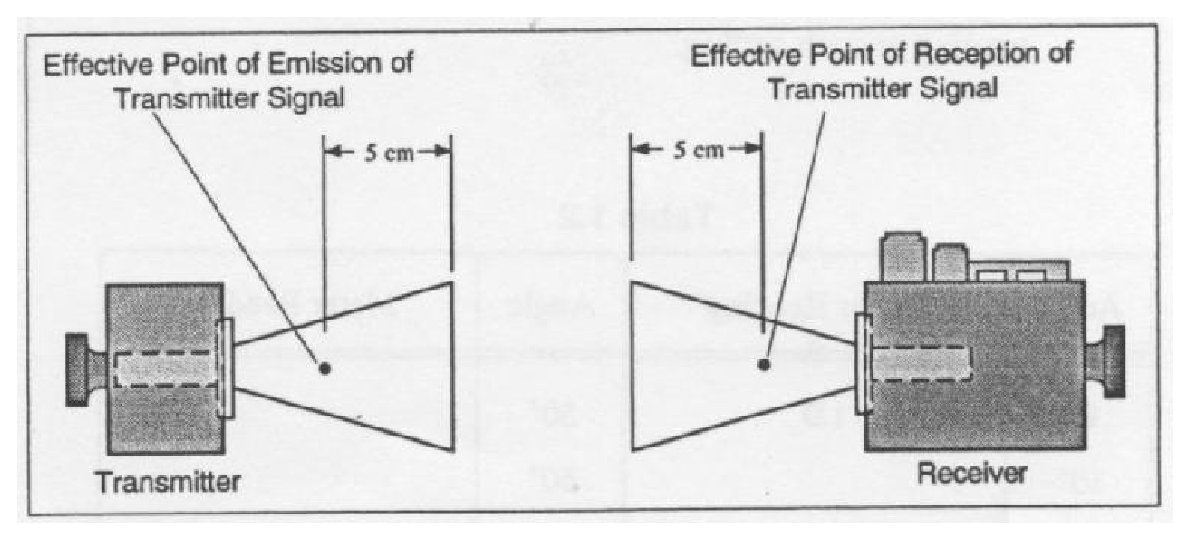
\includegraphics{f23601.eps}}}
\caption{\label{fig:effective}Effective transmission and reception points.}
\end{centering}
\end{figure}

\subsection*{Transmitter}
The transmitter uses a Gunn diode oscillator to produce 15~mW of coherent, linearly polarised microwave radiation. The output is linearly polarised along the axis of the attached horn. The wavelength of the microwaves is about 3 cm. The transmitter is powered from a wall socket. The EM radiation is directed; hence an angle +- 3 degrees other an 180 degrees has significant impact on the readings.



\subsection*{Receiver}

Four ranges are available on the receiver unit, including a variable sensitivity dial. This can be used to offset an initial reading to a convenient value. However, in order to make comparative quantitative measurements, this offset must not be altered between readings. The receiver is powered from internal batteries. To conserve battery power, \textbf{please only turn on when taking measurements and turn off afterwards.}

Note the effective points of transmission and reception in the transmitter and receiver respectively, as shown in Figure \ref{fig:effective}.




It will become apparent that microwaves are easily reflected off a variety of large scale surfaces. For this reason, it is important to note and minimise the effect of reflection of planar surfaces, including walls, the bench-top, the body and any nearby metallic objects.

\section*{Basic Operation}
Before proceeding to the interesting experiments, it is valuable to become familiar with the basic transmitter and receiver system. 



\begin{figure}[!h]
\begin{centering}

\rotatebox{-0.3}{
\scalebox{0.6}{
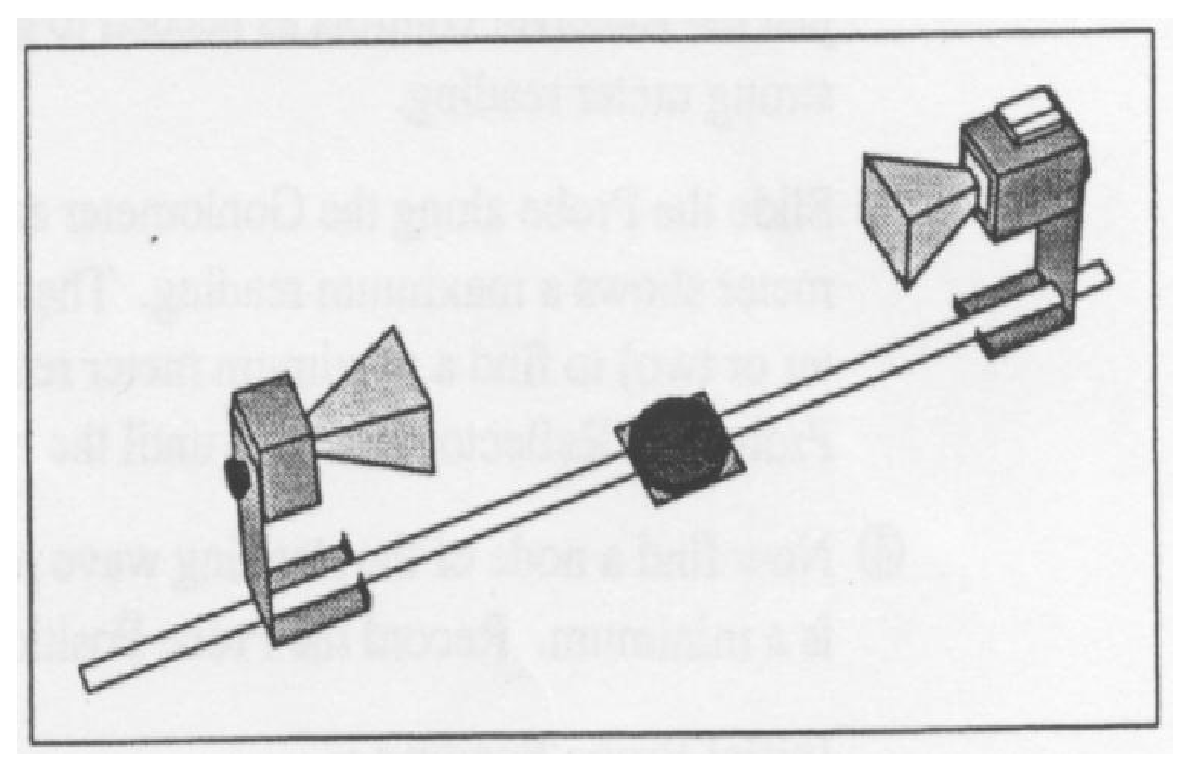
\includegraphics{f23602.eps}}}
\caption{\label{fig:setup}Transmitter and receiver units setup on the goniometer.}
\end{centering}
\end{figure}

\begin{figure}[!h]
\begin{centering}

\rotatebox{-0.3}{
\scalebox{0.6}{
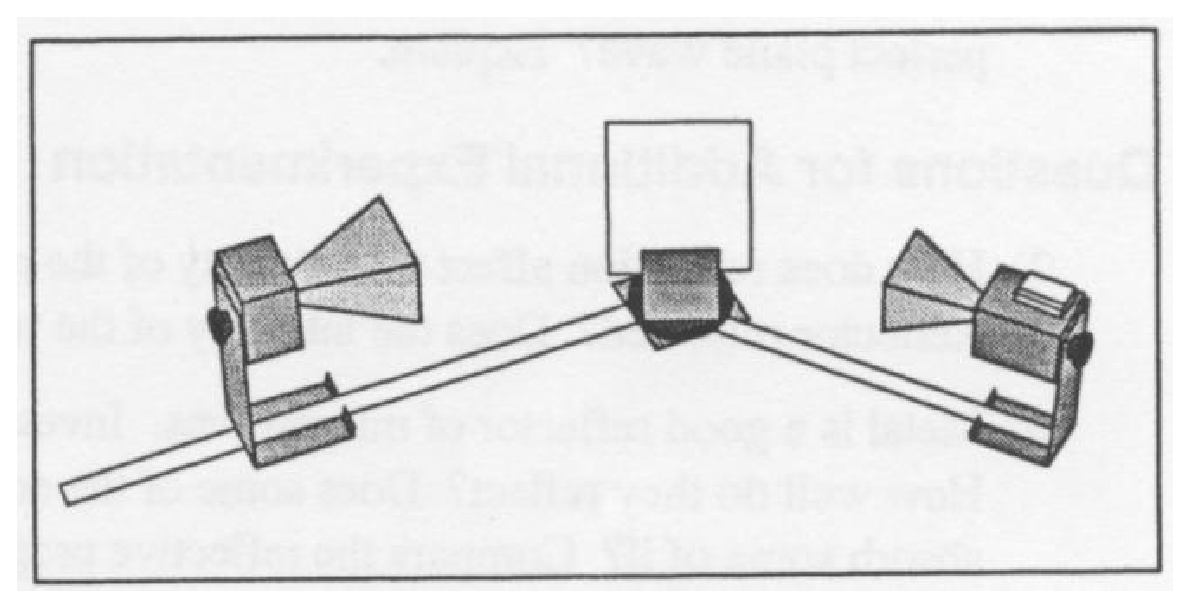
\includegraphics{f23603.eps}}}
\caption{\label{fig:reflection}Setup to verify the principle of reflection.}
\end{centering}
\end{figure}

\begin{enumerate}
\item Place the transmitter and receiver on the \emph{goniometer} (the hinged ruler) with the \textbf{transmitter on the fixed arm}. Set the distance between the transmitter and receiver at \textbf{40cm}. Turn on the transmitter and receiver, and set the receiver controls to show a near full scale deflection. Increase the separation from 40 to 80 cm and record the meter reading in increments corresponding to half the nyquist frequency of the employed wavelength. 

\Question Visualise your readings in a useful manner (e.g. a line plot). Do you think it shows the Intensity $I$ or the amplitude of the electric field $E$; what does the instrument measure? See suggested references for relation between $I$ and $E$.

\Question Determine the wavelength and fit your data qualitatively with a sin-function according to and together with your findings above.

\Question Briefly explain (i.e. not just describe) this behaviour using simplified EM-radiation models (hint: directed vs. undirected radiation)!

\item Beam profile measurements. Place the transmitter such that the end of the output horn is directly over the degree plate. Set the transmitter-receiver distance to about 50cm. Rotate the flexible arm by 5 degree increments up to 90 degrees and record your readings. Visualise your readings in a useful manner. 

\Question Determine the beam width (hint: $1/e$ for $E$ or $1/e2$ for $I$). 

\Question Explain the nature of your findings in less than 50 words! 


\item Reflection and transmission. Angle the \emph{goniometer} to 135 degrees. Sepate transmitter and receiver to 40 cm each side. Place a reflector (metal, then wood) onto the joint in-line to the transmitter EM radiation axis. rotate the reflector from 0 to 45 degrees to steer the beam across the receiver. Record and visualise your readings appropriately. Repeat with a \emph{goniometer} angle of 180 degrees.  

\Question Determine a) reflection and b) transmisison coefficients for 1) metal and 2) wood. 

\Question Explain the nature of your findings in less than 100 words!



\section*{Polarisation}

In this part of the experiment, the polarisation properties of the microwave beam will be investigated. The microwave beam is linearly polarised along the transmitter diode axis, see Figure \ref{fig:polarization}. Similarly, the receiver diode only detects the component of the incident microwave field that is parallel to its axis.
\begin{figure}[!h]
\begin{centering}

\rotatebox{0}{
\scalebox{0.5}{
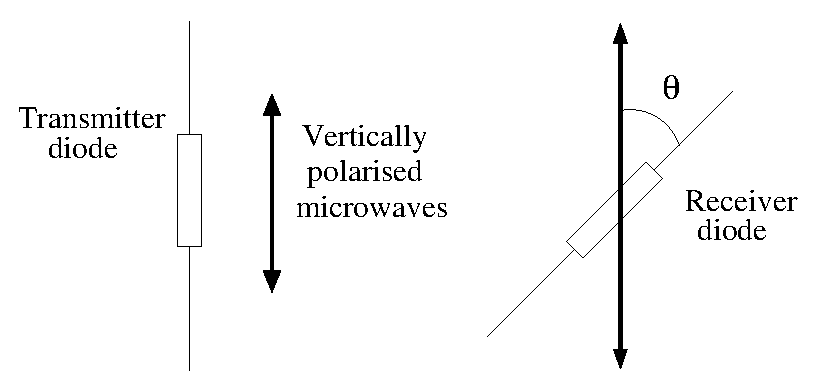
\includegraphics{f23605.eps}}}
\caption{\label{fig:polarization}Detecting polarized radiation.}
\end{centering}
\end{figure}
  

\item Arrange the transmitter and receiver units to be directly facing each other at a distance of about 60cm. Ensure that the horn on each unit has the same orientation, e.g. both horizontal or vertical.  Loosen the hand-screw at the back of the transmitter unit and rotate the unit in increments of 10 degrees. Record the receiver meter reading. Plot the meter reading against polarisation angle.

\item Repeat previous step but now place the metal panel/plate in between sender and receiver (magnetic mount), so that it is inline (not perpendicular to the beam) and rotate both sender and receiver simultaniously and take reading each step. 

\Question Think critically. What do you a) expect, b) observe and c) why exactly do EM waves give you these different readings? Hint: Dipole atenna radiation and polarisation / EM radiation.  (about 100 words)



\subsection*{Brewster's Angle}

In this experiment, Brewster's angle for microwaves will be determined. 

\item Set up the goniometer with the receiver unit on the rotating arm. Place the rotating table on the degree plate. Place the polyethylene
panel on the rotating table. See Figure \ref{fig:brewster}. Set the angle of incidence to 20 degrees and observe at the same angle  (i.e.
140 degrees from the straight through position). Ensure that both the transmitter and receiver units are set for horizontal polarisation.
Set the receiver controls for a half full scale reading. Record the meter reading. Carefully rotate both the receiver and transmitter units
for vertical polarisation. 

\Question Record the meter reading. What does it tell you? 10-30 Words

\begin{figure}[!h]
\begin{centering}

\rotatebox{0}{
\scalebox{0.6}{
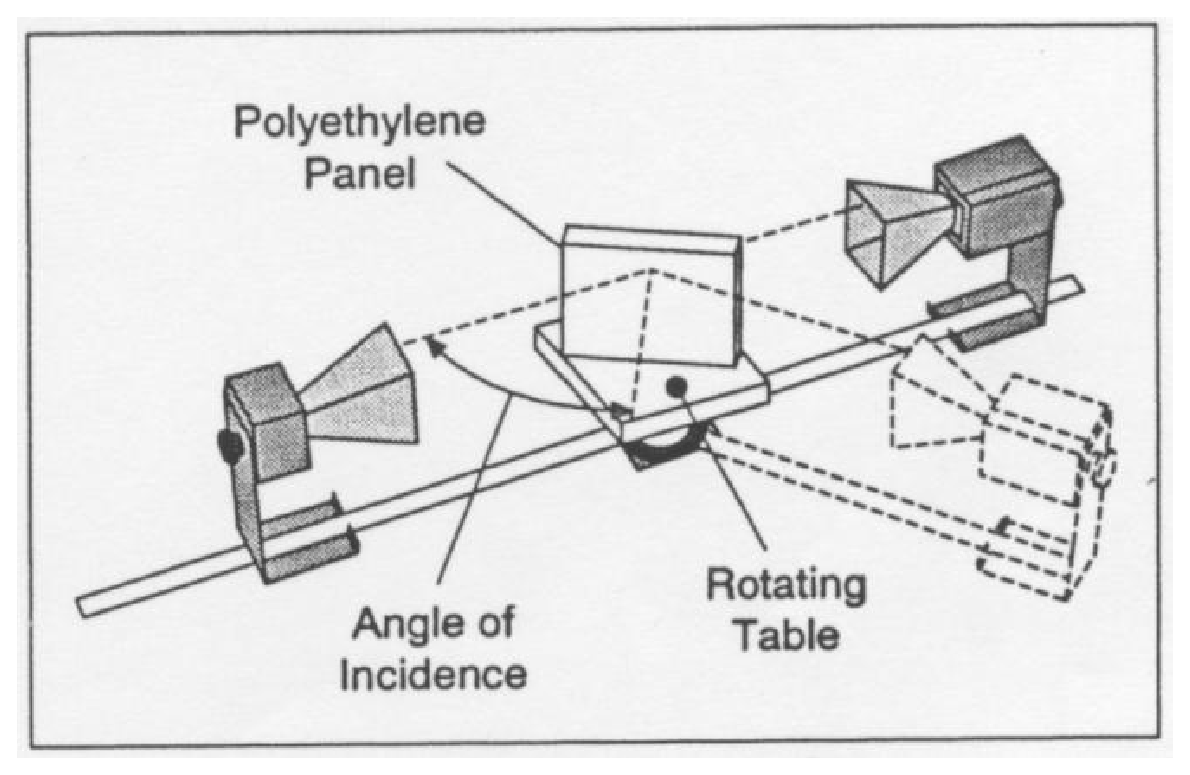
\includegraphics{f23606.eps}}}
\caption{\label{fig:brewster}Set-up for the measurement of Brewster's angle}
\end{centering}
\end{figure}

\item Increase the angle of incidence in regular steps up to about 75 degrees. For each angle of incidence, observe at the same angle and
record the meter reading for the reflected beam for both horizontal and vertical polarisations. You may need to change the receiver
sensitivity. Remember, do not alter the variable sensitivity dial.

\Question  Plot a graph of the meter reading against incident angle for both vertical and horizontal polarisations. You should be able to identify Brewster's angle (where a horizontally polarised wave does not reflect). Make further readings for angles around this value. Plot your whole data set. Why do you observe this (cause)? (less than 100 words)

\Question If you find 43.6 degrees. What index of refraction does it corrspond to? 

\subsection*{Total and Frustrated Total Internal Reflection}

The goals of this experiment are: (i) To find the refractive index of wax to microwaves, (ii) observe total internal reflection and (iii) frustrated internal reflection. This experiment calls for the use of wax prisms. Handle the wax prisms gently, as the wax is brittle and will shatter if dropped.

\item Use one of the wax prisms to demonstrate total internal reflection. Describe in detail how you demonstrated the phenomenon of total internal reflection, see Figure \ref{fig:prism1}.

\begin{figure}[!h]
\begin{centering}

\rotatebox{0}{
\scalebox{0.6}{
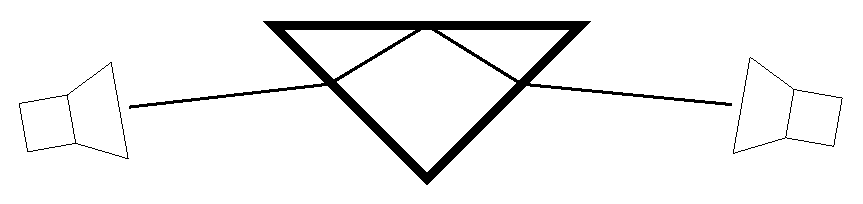
\includegraphics{f23607.eps}}}
\caption{\label{fig:prism1}Total internal reflection of microwaves through the wax prism.}
\end{centering}
\end{figure}

\item Dismantle the apparatus used above. Take the transmitter and receiver units off their metal stands. Arrange the transmitter, receiver and a prism on the table top such that total internal reflection is occurring. Place the transmitter about 20 cm away from the prism. Check that total internal reflection is occurring by bringing the receiver right up against the hypotenuse face of the prism. With the second prism, place the receiver hard up against one of the (equal length) faces. Move the receiver and the second prism as one slowly towards the first prism, as in Figure \ref{fig:prism2}. Keep the hypotenuse faces of the prisms parallel. Monitor the meter reading. Continue until the hypotenuse faces nearly contact. 

\Question What happens? Explain your observations. (less than 100w)

\item Arrange the prisms like in Figure \ref{fig:prism2}. Close the prisms and separate the Prism 1 from Prism 2 in in 1 cm steps up to 10 cm. Record your readings.

\Question Determine the distribution of the evanescent field empertically and compare with your theoretical prediction.

\begin{figure}[!h]
\begin{centering}

\rotatebox{0}{
\scalebox{0.6}{
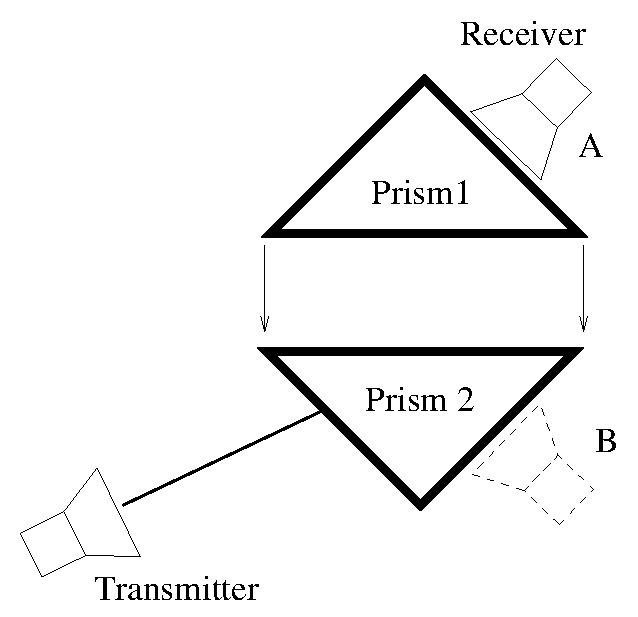
\includegraphics{f23608.eps}}}
\caption{\label{fig:prism2}Frustrated total internal reflection.}
\end{centering}
\end{figure}

\end{enumerate}

\section*{List of Equipment}%

\begin{enumerate}
\item Gunn Diode Transmitter and Receiver units
\item Goniometer
\item 1 component holders
\item 1 metal reflectors (15 cm)
\item 1 partial (wood) reflectors
\item Metal Polariser
\item Rotating foam table
\item Foam prism and quantity of styrene pellets
\item 1 polyethylene blocks
\item 2 wax prisms
\end{enumerate}
\noindent N. Rattenbury \\
\noindent July, 2002.
\end{document}
